\documentclass{standalone}
\usepackage{tikz}
\usetikzlibrary{patterns, positioning}


\begin{document}
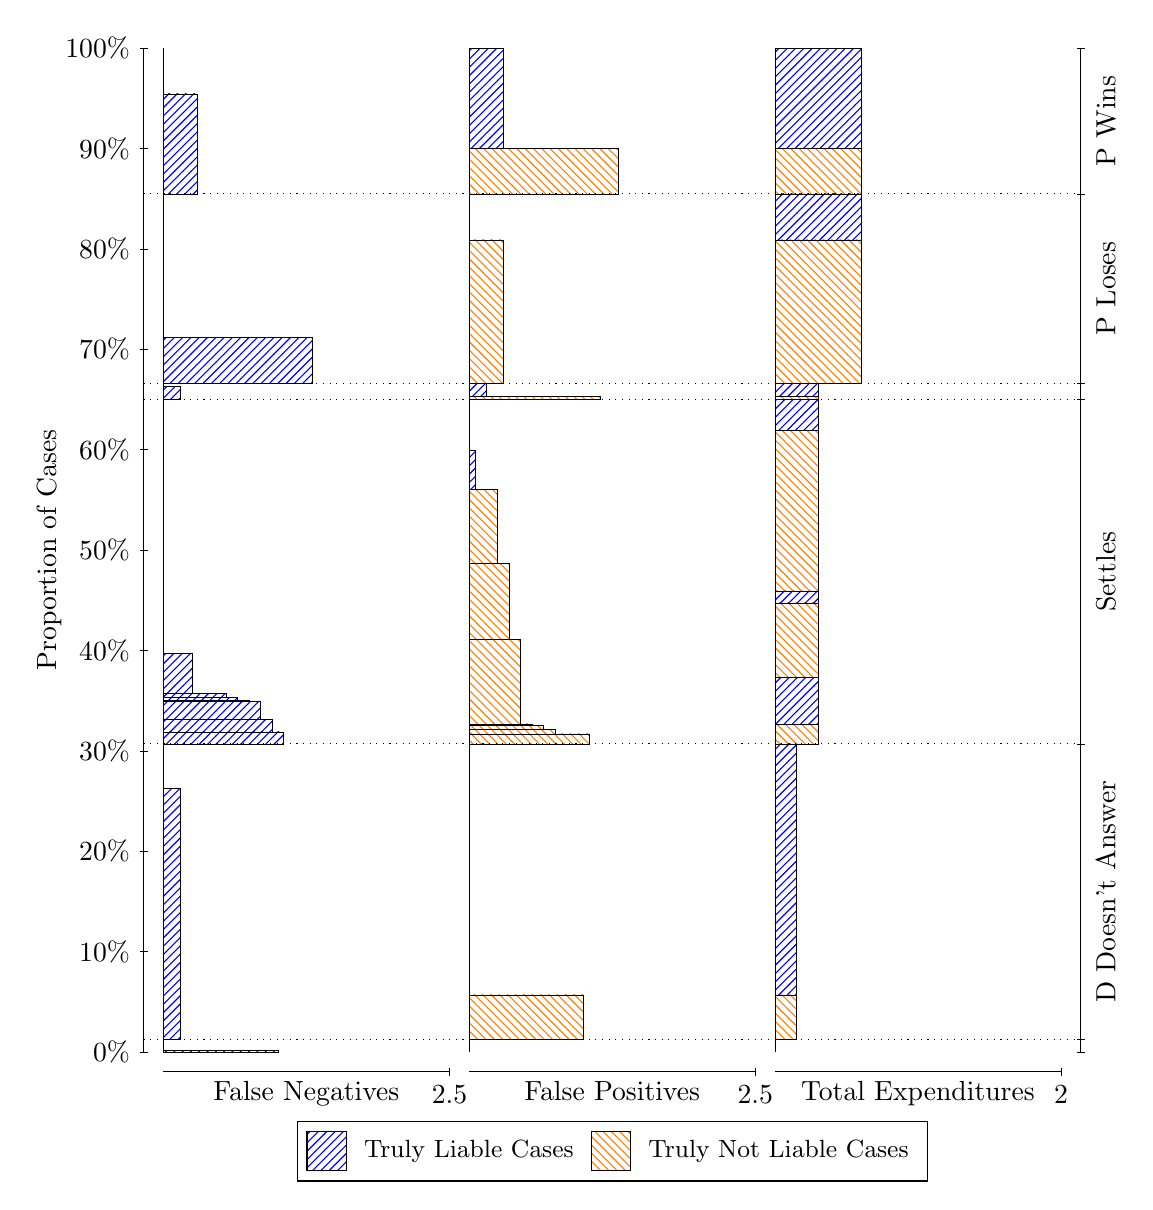
\begin{tikzpicture}
\draw[black, very thin] (1.5,1.75) -- (1.5,14.5);
\node[rotate=90, text=black, anchor=center] at (0.3, 8.125) {Proportion of Cases};
\draw[black, very thin] (1.45,1.75) -- (1.55,1.75);
\node[text=black, anchor=east] at (1.45, 1.75) {0\%};
\draw[black, very thin] (1.45,3.025) -- (1.55,3.025);
\node[text=black, anchor=east] at (1.45, 3.025) {10\%};
\draw[black, very thin] (1.45,4.3) -- (1.55,4.3);
\node[text=black, anchor=east] at (1.45, 4.3) {20\%};
\draw[black, very thin] (1.45,5.575) -- (1.55,5.575);
\node[text=black, anchor=east] at (1.45, 5.575) {30\%};
\draw[black, very thin] (1.45,6.85) -- (1.55,6.85);
\node[text=black, anchor=east] at (1.45, 6.85) {40\%};
\draw[black, very thin] (1.45,8.125) -- (1.55,8.125);
\node[text=black, anchor=east] at (1.45, 8.125) {50\%};
\draw[black, very thin] (1.45,9.4) -- (1.55,9.4);
\node[text=black, anchor=east] at (1.45, 9.4) {60\%};
\draw[black, very thin] (1.45,10.675) -- (1.55,10.675);
\node[text=black, anchor=east] at (1.45, 10.675) {70\%};
\draw[black, very thin] (1.45,11.95) -- (1.55,11.95);
\node[text=black, anchor=east] at (1.45, 11.95) {80\%};
\draw[black, very thin] (1.45,13.225) -- (1.55,13.225);
\node[text=black, anchor=east] at (1.45, 13.225) {90\%};
\draw[black, very thin] (1.45,14.5) -- (1.55,14.5);
\node[text=black, anchor=east] at (1.45, 14.5) {100\%};

\draw[black, very thin] (13.4,1.75) -- (13.4,14.5);
\draw[black, very thin] (13.35,1.75) -- (13.45,1.75);
\node[anchor=west] at (13.35, 1.75) {};
\draw[black, very thin] (13.35,1.9081) -- (13.45,1.9081);
\node[anchor=west] at (13.35, 1.9081) {};
\draw[black, very thin] (13.35,5.6636) -- (13.45,5.6636);
\node[anchor=west] at (13.35, 5.6636) {};
\draw[black, very thin] (13.35,10.037) -- (13.45,10.037);
\node[anchor=west] at (13.35, 10.037) {};
\draw[black, very thin] (13.35,10.244) -- (13.45,10.244);
\node[anchor=west] at (13.35, 10.244) {};
\draw[black, very thin] (13.35,12.647) -- (13.45,12.647);
\node[anchor=west] at (13.35, 12.647) {};
\draw[black, very thin] (13.35,14.5) -- (13.45,14.5);
\node[anchor=west] at (13.35, 14.5) {};

\draw[black, very thin, pattern color=blue, pattern=north east lines] (1.75,1.75) rectangle (3.2033,1.7666);
\draw[black, very thin, pattern color=orange, pattern=north west lines] (1.75,1.7666) rectangle (1.75,1.9081);
\draw[black, very thin, pattern color=blue, pattern=north east lines] (1.75,1.9081) rectangle (1.968,5.0966);
\draw[black, very thin, pattern color=orange, pattern=north west lines] (1.75,5.0966) rectangle (1.75,5.6636);
\draw[black, very thin, pattern color=blue, pattern=north east lines] (1.75,5.6636) rectangle (3.276,5.8156);
\draw[black, very thin, pattern color=blue, pattern=north east lines] (1.75,5.8156) rectangle (3.1307,5.976);
\draw[black, very thin, pattern color=blue, pattern=north east lines] (1.75,5.976) rectangle (2.9853,6.2012);
\draw[black, very thin, pattern color=blue, pattern=north east lines] (1.75,6.2012) rectangle (2.84,6.2168);
\draw[black, very thin, pattern color=blue, pattern=north east lines] (1.75,6.2168) rectangle (2.6947,6.255);
\draw[black, very thin, pattern color=blue, pattern=north east lines] (1.75,6.255) rectangle (2.5493,6.3045);
\draw[black, very thin, pattern color=blue, pattern=north east lines] (1.75,6.3045) rectangle (2.1133,6.8084);
\draw[black, very thin, pattern color=orange, pattern=north west lines] (1.75,6.8084) rectangle (1.75,10.037);
\draw[black, very thin, pattern color=blue, pattern=north east lines] (1.75,10.037) rectangle (1.968,10.206);
\draw[black, very thin, pattern color=orange, pattern=north west lines] (1.75,10.206) rectangle (1.75,10.244);
\draw[black, very thin, pattern color=blue, pattern=north east lines] (1.75,10.244) rectangle (3.6393,10.83);
\draw[black, very thin, pattern color=orange, pattern=north west lines] (1.75,10.83) rectangle (1.75,12.647);
\draw[black, very thin, pattern color=blue, pattern=north east lines] (1.75,12.647) rectangle (2.186,13.917);
\draw[black, very thin, pattern color=orange, pattern=north west lines] (1.75,13.917) rectangle (1.75,14.5);
\draw[black, very thin, pattern color=orange, pattern=north west lines] (5.6333,1.75) rectangle (5.6333,1.8915);
\draw[black, very thin, pattern color=blue, pattern=north east lines] (5.6333,1.8915) rectangle (5.6333,1.9081);
\draw[black, very thin, pattern color=orange, pattern=north west lines] (5.6333,1.9081) rectangle (7.0867,2.4751);
\draw[black, very thin, pattern color=blue, pattern=north east lines] (5.6333,2.4751) rectangle (5.6333,5.6636);
\draw[black, very thin, pattern color=orange, pattern=north west lines] (5.6333,5.6636) rectangle (7.1593,5.7903);
\draw[black, very thin, pattern color=orange, pattern=north west lines] (5.6333,5.7903) rectangle (6.7233,5.8477);
\draw[black, very thin, pattern color=orange, pattern=north west lines] (5.6333,5.8477) rectangle (6.578,5.902);
\draw[black, very thin, pattern color=orange, pattern=north west lines] (5.6333,5.902) rectangle (6.4327,5.9105);
\draw[black, very thin, pattern color=orange, pattern=north west lines] (5.6333,5.9105) rectangle (6.4327,5.9172);
\draw[black, very thin, pattern color=orange, pattern=north west lines] (5.6333,5.9172) rectangle (6.2873,6.9869);
\draw[black, very thin, pattern color=orange, pattern=north west lines] (5.6333,6.9869) rectangle (6.142,7.951);
\draw[black, very thin, pattern color=orange, pattern=north west lines] (5.6333,7.951) rectangle (5.9967,8.8918);
\draw[black, very thin, pattern color=blue, pattern=north east lines] (5.6333,8.8918) rectangle (5.706,9.3957);
\draw[black, very thin, pattern color=blue, pattern=north east lines] (5.6333,9.3957) rectangle (5.6333,10.037);
\draw[black, very thin, pattern color=orange, pattern=north west lines] (5.6333,10.037) rectangle (7.3047,10.075);
\draw[black, very thin, pattern color=blue, pattern=north east lines] (5.6333,10.075) rectangle (5.8513,10.244);
\draw[black, very thin, pattern color=orange, pattern=north west lines] (5.6333,10.244) rectangle (6.0693,12.062);
\draw[black, very thin, pattern color=blue, pattern=north east lines] (5.6333,12.062) rectangle (5.6333,12.647);
\draw[black, very thin, pattern color=orange, pattern=north west lines] (5.6333,12.647) rectangle (7.5227,13.23);
\draw[black, very thin, pattern color=blue, pattern=north east lines] (5.6333,13.23) rectangle (6.0693,14.5);
\draw[black, very thin, pattern color=orange, pattern=north west lines] (9.5167,1.75) rectangle (9.5167,1.8915);
\draw[black, very thin, pattern color=blue, pattern=north east lines] (9.5167,1.8915) rectangle (9.5167,1.9081);
\draw[black, very thin, pattern color=orange, pattern=north west lines] (9.5167,1.9081) rectangle (9.7892,2.4751);
\draw[black, very thin, pattern color=blue, pattern=north east lines] (9.5167,2.4751) rectangle (9.7892,5.6636);
\draw[black, very thin, pattern color=orange, pattern=north west lines] (9.5167,5.6636) rectangle (10.062,5.9105);
\draw[black, very thin, pattern color=blue, pattern=north east lines] (9.5167,5.9105) rectangle (10.062,6.5121);
\draw[black, very thin, pattern color=orange, pattern=north west lines] (9.5167,6.5121) rectangle (10.062,7.4528);
\draw[black, very thin, pattern color=blue, pattern=north east lines] (9.5167,7.4528) rectangle (10.062,7.6048);
\draw[black, very thin, pattern color=orange, pattern=north west lines] (9.5167,7.6048) rectangle (10.062,9.6454);
\draw[black, very thin, pattern color=blue, pattern=north east lines] (9.5167,9.6454) rectangle (10.062,10.037);
\draw[black, very thin, pattern color=orange, pattern=north west lines] (9.5167,10.037) rectangle (10.062,10.075);
\draw[black, very thin, pattern color=blue, pattern=north east lines] (9.5167,10.075) rectangle (10.062,10.244);
\draw[black, very thin, pattern color=orange, pattern=north west lines] (9.5167,10.244) rectangle (10.607,12.062);
\draw[black, very thin, pattern color=blue, pattern=north east lines] (9.5167,12.062) rectangle (10.607,12.647);
\draw[black, very thin, pattern color=orange, pattern=north west lines] (9.5167,12.647) rectangle (10.607,13.23);
\draw[black, very thin, pattern color=blue, pattern=north east lines] (9.5167,13.23) rectangle (10.607,14.5);
\draw[black, dotted] (1.5,1.9081) -- (13.4,1.9081);
\draw[black, dotted] (1.5,5.6636) -- (13.4,5.6636);
\draw[black, dotted] (1.5,10.037) -- (13.4,10.037);
\draw[black, dotted] (1.5,10.244) -- (13.4,10.244);
\draw[black, dotted] (1.5,12.647) -- (13.4,12.647);
\draw[black, very thin] (1.75,1.5) -- (5.3833,1.5);
\node[text=black, anchor=north] at (3.5667, 1.5) {False Negatives};
\draw[black, very thin] (5.3833,1.45) -- (5.3833,1.55);
\node[text=black, anchor=north] at (5.3833, 1.45) {2.5};

\draw[black, very thin] (5.6333,1.5) -- (9.2667,1.5);
\node[text=black, anchor=north] at (7.45, 1.5) {False Positives};
\draw[black, very thin] (9.2667,1.45) -- (9.2667,1.55);
\node[text=black, anchor=north] at (9.2667, 1.45) {2.5};

\draw[black, very thin] (9.5167,1.5) -- (13.15,1.5);
\node[text=black, anchor=north] at (11.333, 1.5) {Total Expenditures};
\draw[black, very thin] (13.15,1.45) -- (13.15,1.55);
\node[text=black, anchor=north] at (13.15, 1.45) {2};


\node[text=black, centered, rotate=90] at (13.72, 3.7858) {D Doesn't Answer};
\node[text=black, centered, rotate=90] at (13.72, 7.8501) {Settles};

\node[text=black, centered, rotate=90] at (13.72, 11.446) {P Loses};
\node[text=black, centered, rotate=90] at (13.72, 13.574) {P Wins};

\draw (7.449999999999999,1.5) node[draw=none] (baseCoordinate) {};
\begin{scope}[align=center]
        \matrix[scale=0.5, draw=black, below=0.5cm of baseCoordinate, nodes={draw}, column sep=0.1cm]{
            \node[rectangle, draw, minimum width=0.5cm, minimum height=0.5cm, pattern color=blue, pattern=north east lines] {}; &
            \node[draw=none, font=\small, text=black] (B) {Truly Liable Cases}; &
            \node[rectangle, draw, minimum width=0.5cm, minimum height=0.5cm, pattern color=orange, pattern=north west lines] {}; &
            \node[draw=none, font=\small, text=black] (B) {Truly Not Liable Cases}; \\
            };
\end{scope}

\end{tikzpicture}
\end{document}